\subsection{Ареновые соединения металлов}
$$PhH_2Cr - D_{6h}$$

\begin{figure}[htp]
\centering
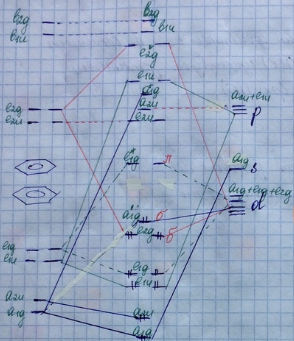
\includegraphics[scale=1.00]{images/DBCrome.png}
\end{figure}

\begin{itemize}
\item $a_{1g}$ взаимодействует с $s$ и $d_z^2$(с первой лучше, так как она более диффузна)
\item $a_{2u}$ с $p_z$ - энергии очень далеки, слабосвяз. и слаборазр.
\item $e_{1g}$ с $d_x^2$ и $d_y^2$($\pi-$связывание, хорошее перекрывание, направлены к $L$)
\item $e_{1u}$ с $p_x, p_y$ - большая разность в энергиях, слабосвяз. и слаборазр., параллельно $L$
\item $e_{2g}$ с $d_{xy}, d_{x^2-y^2}$ ($\sigma-$связывание, параллельно $L$)
\end{itemize}
Особенности:
\begin{itemize}
\item орбитали металла более диффузны, из-за нулевого, в не 2+ заряда, как у Cp
\item L - хороший $\sigma$ и $\pi$ донор
\item $e_{2g}$ связывает сильнее чем в $Cp_2Fe$, из-за лучшего перекрывания(цикл больше), и меньшей разности энергий
\end{itemize}